% !TeX encoding = UTF-8
\documentclass[institutional,screen,none]{../cls/ua-engineering-v6-beamer}
% !TeX encoding = UTF-8
\UASetUniversity{Universidad Austral}
\UASetFaculty{Facultad de Ingeniería}
\UASetDepartment{Departamento de Computación}
\UASetCampus{Pilar}
\UASetCareer{Ingeniería Informática}
\UASetCommission{Comisión A}
\UASetProfessor{Equipo docente}
\UASetSemester{Segundo cuatrimestre 2026}
\UASetCourse{Sistemas Distribuidos}
\UASetDate{2026}


\UASetClassNumber{11}
\UASetClassTitle{Resiliencia distribuida}
\title{\UACourse}
\subtitle{Clase 11 --- Circuit breakers, backpressure, bulkheads, retries y graceful degradation}

\author{\UAProfessor}
\date{\UADate}
\begin{document}

{
\setbeamertemplate{footline}{}
\begin{frame}[plain]
\titlepage
\end{frame}
}

\UASectionSlide{El problema de la falla bajo carga}

\begin{frame}{La intuición equivocada}
Cuando un servicio falla, la reacción intuitiva suele ser:
\begin{itemize}
\item reintentar
\item esperar más
\item escalar horizontalmente
\end{itemize}

\pause

\begin{alertblock}{Problema}
Eso puede empeorar la falla en lugar de resolverla.
\end{alertblock}
\end{frame}

\begin{frame}{Falla local, colapso global}
Escenario típico:
\begin{itemize}
\item una dependencia se vuelve lenta
\item aumentan los timeouts
\item aparecen retries
\item sube la concurrencia
\item se saturan hilos / colas / conexiones
\item el sistema completo colapsa
\end{itemize}
\end{frame}

\begin{frame}{Idea central}
\begin{block}{}
La resiliencia distribuida no consiste en evitar toda falla, sino en impedir que una falla local se propague sin control.
\end{block}
\end{frame}

\UASectionSlide{Retries correctos}

\begin{frame}{Retry: herramienta peligrosa}
Retry puede ser útil para:
\begin{itemize}
\item fallas transitorias
\item pérdidas esporádicas
\item jitter de red
\end{itemize}

\pause

Pero puede ser destructivo ante:
\begin{itemize}
\item saturación
\item fallas persistentes
\item operaciones no idempotentes
\end{itemize}
\end{frame}

\begin{frame}{Buenas prácticas de retry}
\begin{itemize}
\item límite de reintentos
\item exponential backoff
\item jitter
\item solo sobre operaciones idempotentes
\item no reintentar en todas las capas
\end{itemize}
\end{frame}

\UASectionSlide{Circuit Breakers}

\begin{frame}{Circuit Breaker}
\begin{block}{}
Patrón que corta llamadas hacia una dependencia degradada para evitar empeorar la situación.
\end{block}
\end{frame}

\begin{frame}{Estados}
\begin{itemize}
\item Closed
\item Open
\item Half-open
\end{itemize}

\begin{center}
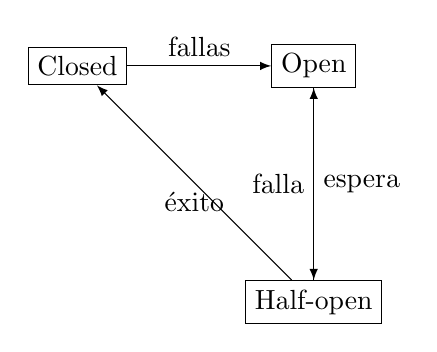
\begin{tikzpicture}[node distance=3cm,>=latex]
\node[draw] (c) {Closed};
\node[draw,right of=c] (o) {Open};
\node[draw,below of=o] (h) {Half-open};

\draw[->] (c) -- node[above]{fallas} (o);
\draw[->] (o) -- node[right]{espera} (h);
\draw[->] (h) -- node[below]{éxito} (c);
\draw[->] (h) -- node[left]{falla} (o);
\end{tikzpicture}
\end{center}
\end{frame}

\begin{frame}{Valor del Circuit Breaker}
\begin{itemize}
\item reduce presión sobre dependencia fallando
\item protege recursos locales
\item acelera feedback de error
\end{itemize}
\end{frame}

\UASectionSlide{Backpressure}

\begin{frame}{Backpressure}
\begin{block}{}
Mecanismo para limitar o regular la producción cuando el consumidor no puede sostener el ritmo.
\end{block}
\end{frame}

\begin{frame}{Sin backpressure}
\begin{itemize}
\item colas crecen
\item memoria se agota
\item latencia explota
\item timeouts disparan retries
\end{itemize}
\end{frame}

\begin{frame}{Con backpressure}
\begin{itemize}
\item se desacelera la entrada
\item se rechaza o posterga trabajo
\item se preserva estabilidad
\end{itemize}
\end{frame}

\UASectionSlide{Bulkheads}

\begin{frame}{Bulkheads}
\begin{block}{}
Aislar recursos para que la saturación de un componente no arrastre a todos los demás.
\end{block}
\end{frame}

\begin{frame}{Ejemplos}
\begin{itemize}
\item pools de hilos separados
\item colas independientes
\item límites por tenant
\item presupuestos de concurrencia
\end{itemize}
\end{frame}

\UASectionSlide{Graceful Degradation}

\begin{frame}{Graceful Degradation}
\begin{block}{}
Cuando el sistema no puede entregar el servicio completo, entrega una versión degradada pero útil.
\end{block}
\end{frame}

\begin{frame}{Ejemplos}
\begin{itemize}
\item mostrar catálogo sin recomendaciones
\item aceptar lectura pero no escritura
\item servir cache vieja
\item omitir features secundarias
\end{itemize}
\end{frame}

\UASectionSlide{Diseño integrado}

\begin{frame}{Patrones combinados}
La resiliencia real suele combinar:
\begin{itemize}
\item timeouts
\item retries limitados
\item circuit breakers
\item backpressure
\item bulkheads
\item degradación elegante
\end{itemize}
\end{frame}

\begin{frame}{Pregunta correcta}
No es:
\begin{quote}
“¿Cómo hago para que nunca falle?”
\end{quote}

\pause

Es:
\begin{quote}
“¿Cómo hago para que falle de forma contenida, comprensible y recuperable?”
\end{quote}
\end{frame}

\UASectionSlide{Cierre}

\begin{frame}{Idea central}
\begin{block}{}
La resiliencia distribuida es control de propagación de falla, no negación de la falla.
\end{block}
\end{frame}

\end{document}
